\section{CIC up-sampler}
    \label{CIC up-sampler}
    \newcommand*{\XNAF}{X_\text{NAF}}
    \newcommand*{\YNAF}{Y_\text{NAF}}
    \newcommand*{\tYNAF}{\tilde{Y}_\text{NAF}}
    \newcommand*{\XNF}{X_\text{NF}}
    \newcommand*{\YNF}{Y_\text{NF}}
    \newcommand*{\tYNF}{\tilde{Y}_\text{NF}}
    FPGA, ASIC による実装を前提として加算器(組み合わせ論理回路)の直後に Flip-flop を置く。
    Web 情報の多くはこれによる遅延を考慮しておらず,本書の結果と異なる数式を導いているが,影響があるのは遅延量だけであり,本質は変わらない。
    \par
    次の図は CIC up-sampler のブロック図である。
    $R\in\naturalNumbers$ はアップ・サンプリング・レートを表し,$M\in\naturalNumbers$ は差分器のホップ数,$N\in\naturalNumbers$ は差分器と積算器それぞれの段数を表す。
    \begin{figure}[H]
        \centering
        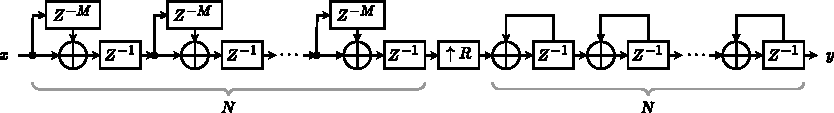
\includegraphics[keepaspectratio, scale=1]
        {\currfiledir/figs/CIC_up-sampler.pdf}
        \caption{CIC up-sampler のブロック図}
    \end{figure}
    \subsection{周波数スペクトラム}
        \label{CIC up-sampler の周波数スペクトラム}
        差分器 1 つの漸化式は $y(n) = x(n-1) - x(n-1-M)$ であり,伝達関数は $(z^{-1})(1-z^{-M})$ である。
        ここに $x,y:\integers\to\complexNumbers$ は差分器への入力と出力である。
        同様に記号を流用して積算器の入出力 1 つの漸化式は $y(n) = y(n-1) + x(n-1)$ であり,伝達関数は $(z^{-1})/(1-z^{-1})$ である。
        Noble Identity を用いて $R$ 倍オーバー・サンプラを最前段に移動すると, $R$ 倍オーバー・サンプラの後ろの伝達関数は次式である。
        \[ H_\text{C,I}(z) = z^{-N(R+1)}\parens*{\frac{1-z^{-MR}}{1-z^{-1}}}^N = z^{-N(R+1)}\parens*{\sum_{n=0}^{MR-1} z^{-n}}^N \]
        (C, I はそれぞれ comb, integrator の意味)これは,長さ $MR$ の区間の和をとるブロックを $N$ 段従属接続して $N(R+1)$ だけ遅延させる操作と等価である。
        この系に対して元の信号を $MR$ 倍にオーバー・サンプルした信号を入力して得られる出力が CIC up-sampler の出力である。
        \par
        CIC up-sampler の出力の絶対値が最大となるのは,入力のビット幅が許す範囲の絶対値最大(この値を $x_\text{MAX}$ とおく)の定数列が入力された場合であり,値は次式である。
        \begin{equation}
            x_\text{MAX}(MR)^{N-1}
            \label{equation:CIC up-sampler の出力の絶対値の最大値}
        \end{equation}
        このことから直ちに解るが, CIC up-sampler の直流ゲインは $(MR)^{N-1}$ である。
        \par
        入力と出力の DTFT をそれぞれ $\XNAF(\Omega), \YNAF(\Omega)$ ($\Omega$ は正規化角周波数) とする。
        $H_\text{C,I}(z)$ に於いて $z = \exp(i\Omega)$ とし,\ref{オーバー・サンプリングされた信号の DTFT} を適用し,周波数スペクトラムとして次式を得る。
        \begin{align*}
            \YNAF(\Omega) &= \exp(-iN(R+1)\Omega)\frac{\parens*{1-\exp\parens*{-iMR\Omega}}^N}{\parens*{1-\exp\parens*{-i\Omega}}^N}\XNAF(R\Omega) \\
            &= \exp\parens*{-i\frac{\Omega}{2}N((M+2)R+1)}\parens*{\frac{\sin(MR\Omega/2)}{\sin(\Omega/2)}}^N \XNAF(R\Omega)
        \end{align*}
        正規化周波数で表現しなおして $\XNF(F) = \XNAF(2\pi F), \YNF(F) = \YNAF(2\pi F)$ とすれば次式を得る。
        \begin{align}
            \YNF(F) &= \exp\parens*{-i\frac{2\pi F}{2}N((M+2)R+1)}\parens*{\frac{\sin(MR 2\pi F/2)}{\sin(2\pi F/2)}}^N \XNF(RF) \nonumber \\
            &= \exp\parens*{-i\pi N((M+2)R+1)F}\underbrace{\parens*{\frac{\sin(\pi MRF)}{\sin(\pi F)}}^N}_{(1)} \XNF(RF) \label{equation:CIC up-sampler の周波数スペクトラム}
        \end{align}
        この式は $F\to 0$の極限で $R^N \XNF(0)$ となる。
        しかし入力を直流としたときに出力の絶対値が $R^N$ 倍になるわけではない。
        なぜならば既に述べたように, Noble Identity を用いて移動したオーバー・サンプラが,伝達関数に含まれる長さ $R$ の区間和の 1 つと相殺するからである。
        周波数スペクトラムと「振幅特性」(すぐ後に明かされるように,この単語は正しく定義されないので敢えて「」付きで示した)が一致しない原因は単純で,オーバー・サンプルという非線形な操作を加えた結果,正弦波入力に対する出力が正弦波とならないからである。
        この状況では「振幅特性」自体が定義できない。
        アップ・サンプルによって正弦波が緻密になって出力されたように見えても,それは「そう見える」だけであり,厳密には正弦波ではなく広がりをもったスペクトラムをもつ信号に変わっている。
        \par
        式 \eqref{equation:CIC up-sampler の周波数スペクトラム} の伝達関数部分の特性をプロットする際に (1) の分母の零点が厄介である。
        分子を見ると解るが,分母と分子の零点の位数がともに 1 であり相殺する(可除特異点)ため,全体としては有界である。
        この特異点は整数($k$ とする)にあり,簡単な計算によって $F=k$ のとき $(1) = [(-1)^{(MR-1)k} MR]^N$ であることが確かめられる。
        プログラムでは $\sin\pi F$ が小さいときに近似式に切り替えることで 0 除算を回避できる。
    \subsection{差分器と積算器に必要なビット幅}
        \subsubsection{差分器のビット幅}
            差分器の出力の絶対値が最大となるのは,入力のビット幅が許す範囲の最大振幅で周期 $2M$ の交代列が入力されるときである。
            よって,差分器の出力のビット幅は入力のそれの 2 倍を確保すればよく,$N$ 段目の差分器の出力のビット幅は初段の入力のビット幅 + $N$ とすればよい。
        \subsubsection{積算器のビット幅(解析的な方法)}
            CIC up-sampler の入力のビット幅を $B$ とする。
            まず,\cref{equation:CIC up-sampler の出力の絶対値の最大値} より最終段の積算器(第 $N$ 積算器)の出力のビット幅は $B + (N-1)\log_2 MR$ を確保すれば必要十分である。
            \par
            最終段より前の積算器については必要十分なビット幅を解析的に求めることはできないが,十分な値であれば次のようにして求められる。
            \par
            第 $(N-1)$ 積算器の出力のビット幅を考える。
            第 $2$ 差分器から第 $(N-1)$ 積算器までに注目すると,これはステージ数 $N-1$ の CIC up-sampler となっている。
            このことと,元の第 $1$ 差分器の出力の絶対値の最大値がビット幅 $B+1$ で収容できることから,第 $(N-1)$ 積算器の出力はビット幅 $B + 1 + (N-2)\log_2 MR$ を確保すれば十分である。
            (元の第 $1$ 差分器の出力が最大値で一定していることはあり得ないことは容易に解る。
            この点を無視して上限で評価しており,故に「必要な」ビット幅からの乖離がある。)
            \par
            同様にして次々に内側の小さい CIC up-sampler を考えてゆくと,十分なビット幅が求まる。
            $MR\geq 2$ であるから,内側は外側に比べてビット幅が小さいかまたは等しい。
        \subsubsection{積算器のビット幅(数値的な方法)}
            最終段については既に述べたように解析的に求められるのでここでは扱わない。
            \par
            Noble Identity を用いて $R$ 倍オーバー・サンプラを最前段に移動した後,第 1 差分器から第 $n\in\{1,2,...,N-1\}$ 段の積算器までの部分系の伝達関数を考えると次式を得る。
            \[ \frac{(1-z^{-MR})^N}{(1-z^{-1})^n} = (1-z^{-MR})^{N-n}\parens*{\sum_{n=0}^{MR-1} z^{-n}}^n \]
            上式のうち,$\sum_{n=0}^{MR-1} z^{-n}$ 1 つ分については,この系の前段に移動された $R$ 倍オーバー・サンプラと相殺し,ビット幅増加に寄与しない。
            よって,ビット幅の増加に寄与する部分は次式である。
            \begin{equation}
                (1-z^{-MR})^{N-n}\parens*{\sum_{n=0}^{MR-1} z^{-n}}^{n-1} = \frac{(1-z^{-MR})^{N-1}}{(1-z^{-1})^{n-1}} \label{equation:CIC up-sampler の部分系の伝達関数}
            \end{equation}
            これは抽出された部分系の有限インパルス応答の z 変換である。
            この系の応答の絶対値が最大となるような作為的な入力に対する応答を収容できるビット幅を確保すればよい。
            そのような最悪の応答は \cref{equation:CIC up-sampler の部分系の伝達関数} を計算機代数システムを用いて $z^{-1}$ の多項式として展開し,係数の絶対値の総和をとることで得られる。
    \subsection{CIC up-sampler 補償フィルタ}
        \newcommand*{\HCNF}{H_\text{C,NF}}
        \cref{equation:CIC up-sampler の周波数スペクトラム} より,アップ・サンプリングにより $\XNF$ には $F$ に依存する因子が掛かる。
        これをできるだけ補正するために,CIC up-sampler の直前で前記の因子の逆特性を近似する feedforward フィルタ(以下単に「FIR フィルタ」と呼ぶ)の適用を考える。
        このフィルタの周波数スペクトラムを $\HCNF$ とすると次式が成り立つ。
        \[ \YNF(F) = \exp\parens*{-i\pi N((M+2)R+1)F}\parens*{\frac{\sin(\pi MRF)}{\sin(\pi F)}}^N \HCNF(RF)\XNF(RF) \]
        $\HCNF(F)$ に求められるのは $F \in [-1/2,1/2]$ の範囲で次式を近似することである。
        \begin{equation}
            \exp\parens*{i\pi N\frac{(M+2)R+1}{R}F}\parens*{\frac{\sin(\pi F/R)}{\sin(\pi MF)}}^N \label{equation:CIC up-sampler 補償フィルタの理想的な周波数スペクトラム}
        \end{equation}
        $R$ が大きいとき,$\sin(\pi F/R) \sim \pi F/R$ として \cref{equation:CIC up-sampler 補償フィルタの理想的な周波数スペクトラム} の振幅特性が $(MR\sinc(\pi MF))^{-N}$ に漸近する。
        \par
        $\HCNF$ が周期 1 の関数であることから, $[-1/2,1/2]$ の区間全体で上式を近似することはできない(端点で微分不可能になる)。
        現実には,$\alpha[-1/2,1/2]\;(0<\alpha<1)$ の範囲を Remez のアルゴリズム等で近似する。
        $\alpha$ が 1 に近づく程,必要な係数が増える。
        \cref{equation:CIC up-sampler の周波数スペクトラム} が示すように CIC up-sampler の位相特性が線形なので Remez のアルゴリズムでは振幅の補正だけを気にして係数設計してよい(生成される FIR フィルタの位相特性も線形なので合成系の位相特性も線形となる)。
        \par
        アップ・サンプリングを全て CIC up-sampler で行うのではなく,一部を CIC up-sampler の前段にオーバー・サンプラと帯域制限用 FIR フィルタ(「FIR フィルタ 1」と呼ぶ)の組を置いてそれに分担させ,FIR フィルタ 1 に後段の CIC up-sampler の補正フィルタを兼任させる(合成する)こともしばしば行われる。
        例えば, FIR フィルタ 1 の直前で 2 倍アップ・サンプリングを行う場合,FIR フィルタ 1 では $0.8\times[-1/4,1/4]$ の領域で \cref{equation:CIC up-sampler 補償フィルタの理想的な周波数スペクトラム} を近似し,$[-1/2,-1.2\times(1/4)-]\cup[1.2\times(1/4),1/2]$ の領域を阻止帯とするように Remez のアルゴリズムで係数を計算する。
\section{CIC down-sampler}
    \ref{CIC up-sampler} と同様に加算器(組み合わせ論理回路)の直後に Flip-flop を置く。
    次の図は CIC down-sampler のブロック図である。
    $R\in\naturalNumbers$ はダウン・サンプリング・レートを表し,$M\in\naturalNumbers$ は差分器のホップ数,$N\in\naturalNumbers$ は差分器と積算器それぞれの段数を表す。
    \begin{figure}[H]
        \centering
        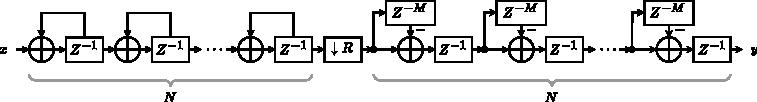
\includegraphics[keepaspectratio, scale=1]
        {\currfiledir/figs/CIC_down-sampler.pdf}
        \caption{CIC down-sampler のブロック図}
    \end{figure}
    \subsection{周波数スペクトラム}
        Noble Identity を用いて $1/R$ 倍アンダー・サンプラを最終段に移動すると,\ref{CIC up-sampler の周波数スペクトラム} と同様にして, $1/R$ 倍アンダー・サンプラより前の伝達関数は次式である。
        \[ H_\text{I,C}(z) = z^{-N(R+1)}\parens*{\frac{1-z^{-MR}}{1-z^{-1}}}^N = z^{-N(R+1)}\parens*{\sum_{n=0}^{MR-1}z^{-n}}^N \]
        (C, I はそれぞれ comb, integrator の意味)これは,長さ $MR$ の区間の和をとるブロックを $N$ 段従属接続して $N(R+1)$ だけ遅延させる操作と等価である。
        この系の出力を $1/R$ でアンダー・サンプルした結果が CIC down-sampler の出力である。
        よって,系の出力の絶対値が最大となるのは,絶対値が最大の定数 ($x_\text{MAX}$ とする)を入力し続けたときであり,そのときの出力の絶対値は $(MR)^N x_\text{MAX}$ である。
        このことから直ちに解るが,直流ゲインは $(MR)^N$ である。
        \par
        入力の DTFT を $\XNAF(\Omega)$ ($\Omega$ は正規化角周波数) とする。
        $1/R$ 倍アンダー・サンプラより前の出力の DTFT を $\tYNAF(\Omega)$ とする。
        $H_\text{I,C}(z)$ に於いて $z = \exp(i\Omega)$ とすると次式が成り立つ。
        \begin{align*}
            \tYNAF(\Omega) &= \exp(-iN(R+1)\Omega)\frac{\parens*{1-\exp\parens*{-iMR\Omega}}^N}{\parens*{1-\exp\parens*{-i\Omega}}^N}\XNAF(\Omega) \\
            &= \exp\parens*{-i\frac{\Omega}{2}N((M+2)R+1)}\parens*{\frac{\sin(MR\Omega/2)}{\sin(\Omega/2)}}^N \XNAF(\Omega)
        \end{align*}
        正規化周波数で表現しなおして $\XNF(F) = X(2\pi F), \tYNF(F) = \tYNAF(2\pi F)$ とすれば次式を得る。
        \[ \tYNF(F) = \exp\parens*{-i\pi N((M+2)R+1)F}\parens*{\frac{\sin(\pi MRF)}{\sin(\pi F)}}^N \XNF(F) \]
        これと \ref{アンダー・サンプリングされた信号の DTFT} より,$1/R$ 倍アンダー・サンプラの出力を正規化周波数で表現した周波数スペクトラムは次式である。
        \begin{align}
            \YNF(F) &= \frac{1}{R}\sum_{n=0}^{R-1} \tYNF((F-n)/R) \nonumber \\
            &= \frac{1}{R}\sum_{n=0}^{R-1} \exp\parens*{-i\pi N(F-n)\frac{(M+2)R+1}{R}}\parens*{\frac{\sin(\pi M(F-n))}{\sin(\pi(F-n)/R)}}^N \XNF((F-n)/R) \label{equation:CIC down-sampler の周波数スペクトラム}
        \end{align}
        \ref{アンダー・サンプリングされた信号の DTFT} でも述べられているが,全体に掛けられている $1/R$ は DTFT の内積計算の対象となる点の数が $1/R$ に減ったことに由来しており,振幅が $1/R$ になるわけではない。
    \subsection{差分器と積算器に必要なビット幅}
        入力は固定小数点数であるが,全体を適当に2のべき乗倍したものとして見直して符号付整数として扱っても系としては等価なので,以後そうする。
        入力側(サンプル・レートが高い側)から入力される符号付整数のビット幅を $B$ とする。
        \par
        先の議論から,最終段の出力のビット幅は $\ceil{1 + \log_2\parens{(MR)^N 2^{B-1}}} = B + \ceil{N\log_2 MR}$ あれば十分であることが判る。
        \par
        積算器はオーバー・フローし得るが,溢れた桁を捨てる操作が modulo 演算であることと,最終段の出力のビット幅を考えれば,最終段より左側の全ての段のビット幅を最終段と等しくしておけば問題ない(無限のビット幅を持つ仮想的な系と同じ出力が得られる)ことが判る。
    \subsection{CIC down-sampler 補償フィルタ}
        \cref{equation:CIC down-sampler の周波数スペクトラム} より,ダウン・サンプリングにより $\XNF$ には $F$ に依存する因子が掛かる。
        これをできるだけ補正するために,CIC down-sampler の直後で前記の因子の逆特性を近似する feedforward フィルタの適用を考える。
        ダウン・サンプリング後に補償用フィルタを掛けるので,操作できるのは第 1 Nyquist 領域のみである。
        第 1 Nyquist 領域のみを抽出し,補償用フィルタの周波数スペクトラムを $\HCNF$ とすると次式が成り立つ。
        \[ \YNF(F) = \HCNF(F) \frac{1}{R} \exp\parens*{-i\pi N F\frac{(M+2)R+1}{R}}\parens*{\frac{\sin(\pi MF)}{\sin(\pi F/R)}}^N \XNF(F/R) \]
        $\HCNF(F)$ に求められるのは $F \in [-1/2,1/2]$ の範囲で次式を近似することである。
        \begin{equation}
            \exp\parens*{i\pi N F\frac{(M+2)R+1}{R}}\parens*{\frac{\sin(\pi F/R)}{\sin(\pi MF)}}^N
        \end{equation}
        この式は偏角の差を除いて \cref{equation:CIC up-sampler 補償フィルタの理想的な周波数スペクトラム} と一致するため,補償用フィルタの設計手法は CIC up-sampler 補償フィルタと同じものを適用できる。
